\section{Index4}
\label{section:Index4}

Index4 uses a new data structure, the hash table, to allow for direct accessing instead of linear searching for a given word. The index uses a hash table of static size $k$ and chained hashing to store the unique words of the input text. Each word in the text is hashed (see equation \ref{eq:hashfunc}) and inserted into the hash table along with its corresponding linked list of articles. In the case of hash collisions, the method of chained hashing simply chains the collided words together in a linked list, see figure \ref{fig:index4hash table}. 

\begin{figure}[ht!]
    \centering
    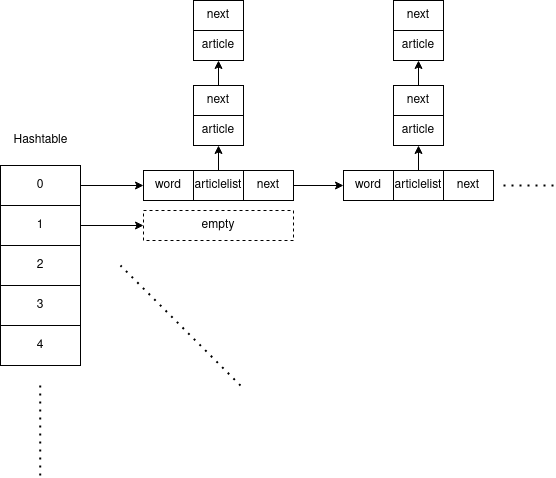
\includegraphics[width=.7\textwidth]{LaTeX/Figures/BasicPart/index4hashtable.png}
    \caption{Illustration of the hash table in Index4 and Index5. Each bucket in the hash table points to the head of a linked list of words that hash to the same value. Each word points to the next word as well as a linked list of the article titles it occurs in.}
    \label{fig:index4hash table}
\end{figure}

The design of a good hash function can be used to avoid too many collisions. A string hash function is a deterministic function that maps strings to numbers, which is used to know where to find a given string in the hash table. One such hash function will map all characters to their corresponding character value as a number. Hereafter all character values will be multiplied with a prime raised to the power of the position of the character in the string. A common prime to use is 31. The hash value is then the sum of all elements. If the hash value is out of bounds for a hash table of a given size, the hash value will lastly be updated to be the remainder after dividing the hash value by the size of the hash table. If the size of the hash table, $k$, is fixed as in this index, it is common for $k$ to also be a prime number as this can reduce the number of possible collisions. This described hash function can be written as

\begin{equation}\label{eq:hashfunc}
    H(s)= \sum_{i=1}^{|s|}\left(charValue(s[i])*31^i\right) \mod k
\end{equation}

For a hash table, the worst case would be if all words of the input file were hashed to the same value. In this case, the index would be almost identical to Index3 which checks for unique words in a linked list and uses $O(u\cdot n)$ time. However, assuming a good hash function that spreads words roughly evenly, the expected length of each linked list is $\frac{u}{k}$. The expected time to index is then $O(n\cdot \frac{u}{k})$. When $k$ is chosen wisely, this becomes close to $O(n)$, but for fixed $k$ and large inputs, this equates to $O(n\cdot u)$, like Index3 but with better constants. 

The expected search time of Index4 is $O(\frac{u}{k})$ as it takes constant time to calculate the hash value of the search string and $O(\frac{u}{k})$ time to find the word in the linked list of the hash value. 

The index stores a link for each unique word in the input and its article list, using \\$O(u\cdot a)$ space. Furthermore, the hash table itself takes up $O(k)$ space making it $O(u\cdot a+k)$ space. The search uses only constant, $O(1)$, additional space. 
